\newpage
\section{Web Search}

\subsection{Web Search: Challenges \& Opportunities}
Web search is one of the most important applications of text retrieval.
\begin{itemize}
\item Challenges
\begin{itemize}
\item Scalability (the size of the Web, completeness of coverage, many user queries) $to$ Parallel indexing \& searching (MapReduce)
\item Low quality information and spams $to$ Spam detection \& Robust ranking
\item Dynamics of the Web (new pages are constantly created, some pages may be updated)
\end{itemize}

\item Opportunities
\begin{itemize}
\item many additional heuristics (e.g., link information, layout) can be leveraged to improve search accuracy $to$ Link analysis \& multi-feature ranking
\end{itemize}
\end{itemize}


%---------------------------------------------
\subsection{Basic Search Engine Technologies}
\begin{figure}[H]
    \centering
    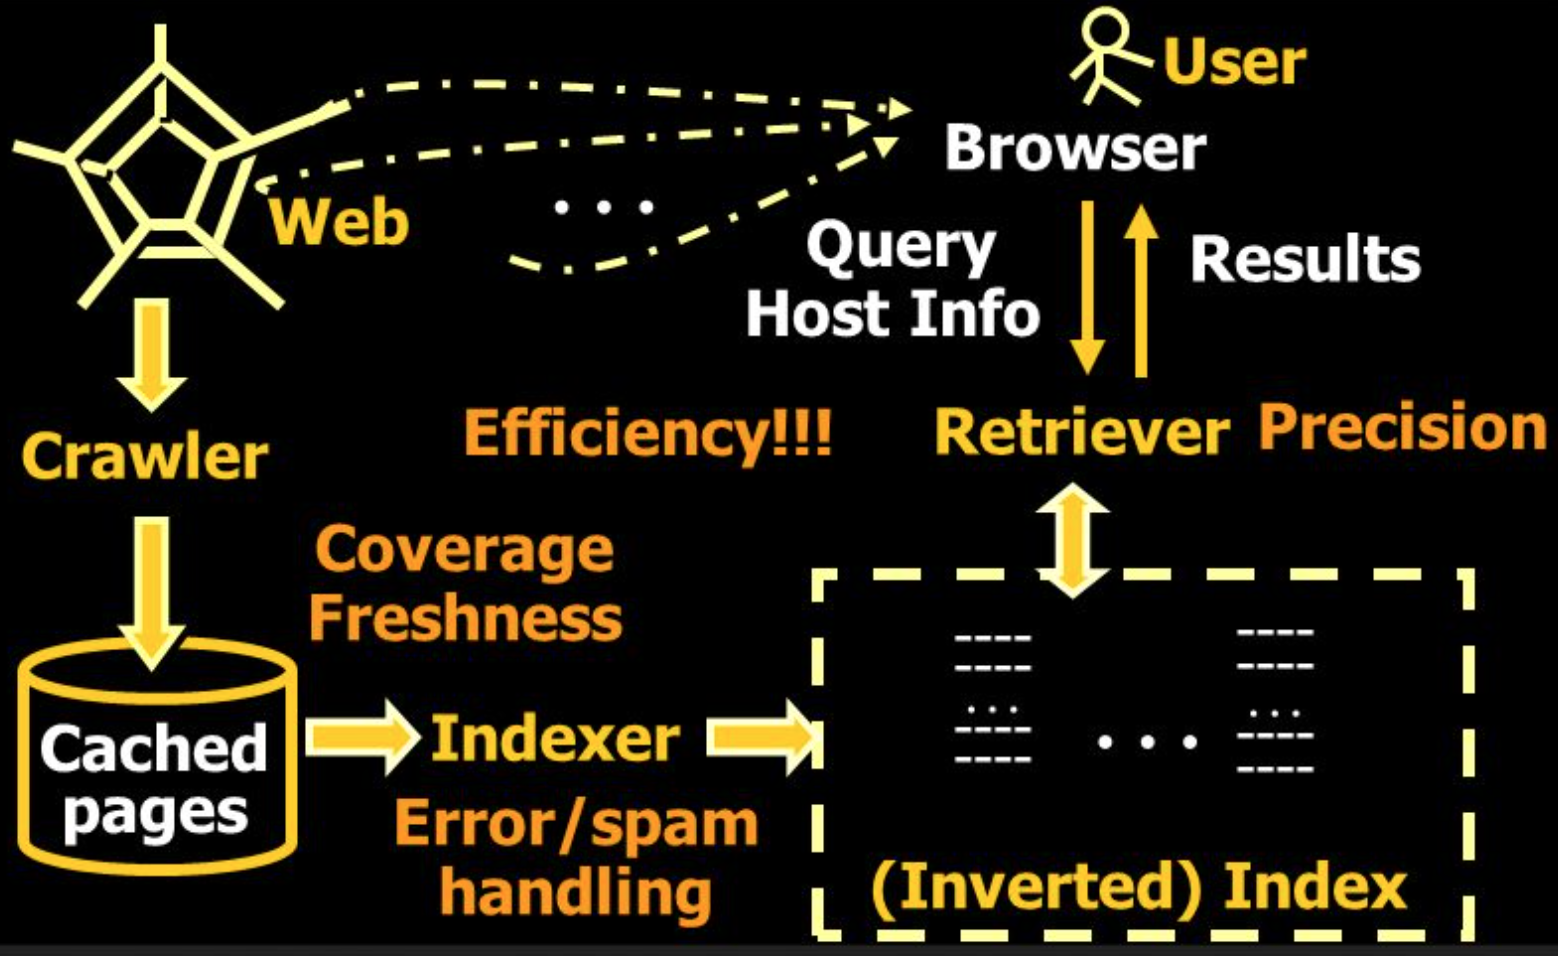
\includegraphics[width=0.9\linewidth]{search_engine.png}
\end{figure}

%---------------------------------------------
\subsection{Crawler/Spider/Robot}

\begin{itemize}
\item Building a <<toy crawler>> is easy
\begin{itemize}
\item Start with a set of “seed pages” in a priority queue
\item Fetch pages from the web
\item Parse fetched pages for hyperlinks; add them to the queue 
\item Follow the hyperlinks in the queue
\end{itemize}

\item A real crawler is much more complicated... 
\begin{itemize}
\item Robustness (server failure, trap, etc.)
\item Crawling courtesy (server load balance, robot exclusion, etc.) 
\item Handling file types (images, PDF files, etc.)
\item URL extensions (cgi script, internal references, etc.)
\item Recognize redundant pages (identical and duplicates)
\item Discover <<hidden>> URLs (e.g., truncating a long URL )
\end{itemize}
\end{itemize}

%--------------
\subsubsection{Major Crawling Strategies}
\begin{itemize}
\item Breadth-First\footnote{\textbf{Breadth-first search (BFS)} is an algorithm for traversing or searching tree or graph data structures. It starts at the tree root (or some arbitrary node of a graph, sometimes referred to as a <<search key>>) and explores the neighbor nodes first, before moving to the next level neighbors.} is common (balance server load)
\item Parallel crawling is natural

\item Variation: focused crawling
\begin{itemize}
\item Targeting at a subset of pages (e.g., all pages about <<automobiles>>) 
\item Typically given a query
\end{itemize}

\item How to find new pages (they may not linked to an old page!)

\item Incremental/repeated crawling
\begin{itemize}
\item Need to minimize resource overhead
\item Can learn from the past experience (updated daily vs. monthly)
\item Target at : 1) frequently updated pages; 2) frequently accessed pages
\end{itemize}
\end{itemize}

%---------------------------------------------
\subsection{Web Index}

Standard IR techniques are the basis, but insufficient – they lack scalability and efficiency. \\

Google’s contributions:
\begin{itemize}
\item Google File System (GFS): distributed file system
\item MapReduce: Software framework for parallel computation 
\item Hadoop: Open source implementation of MapReduce
\end{itemize}

%--------------
\subsubsection{GFS Architecture}
\begin{figure}[H]
    \centering
    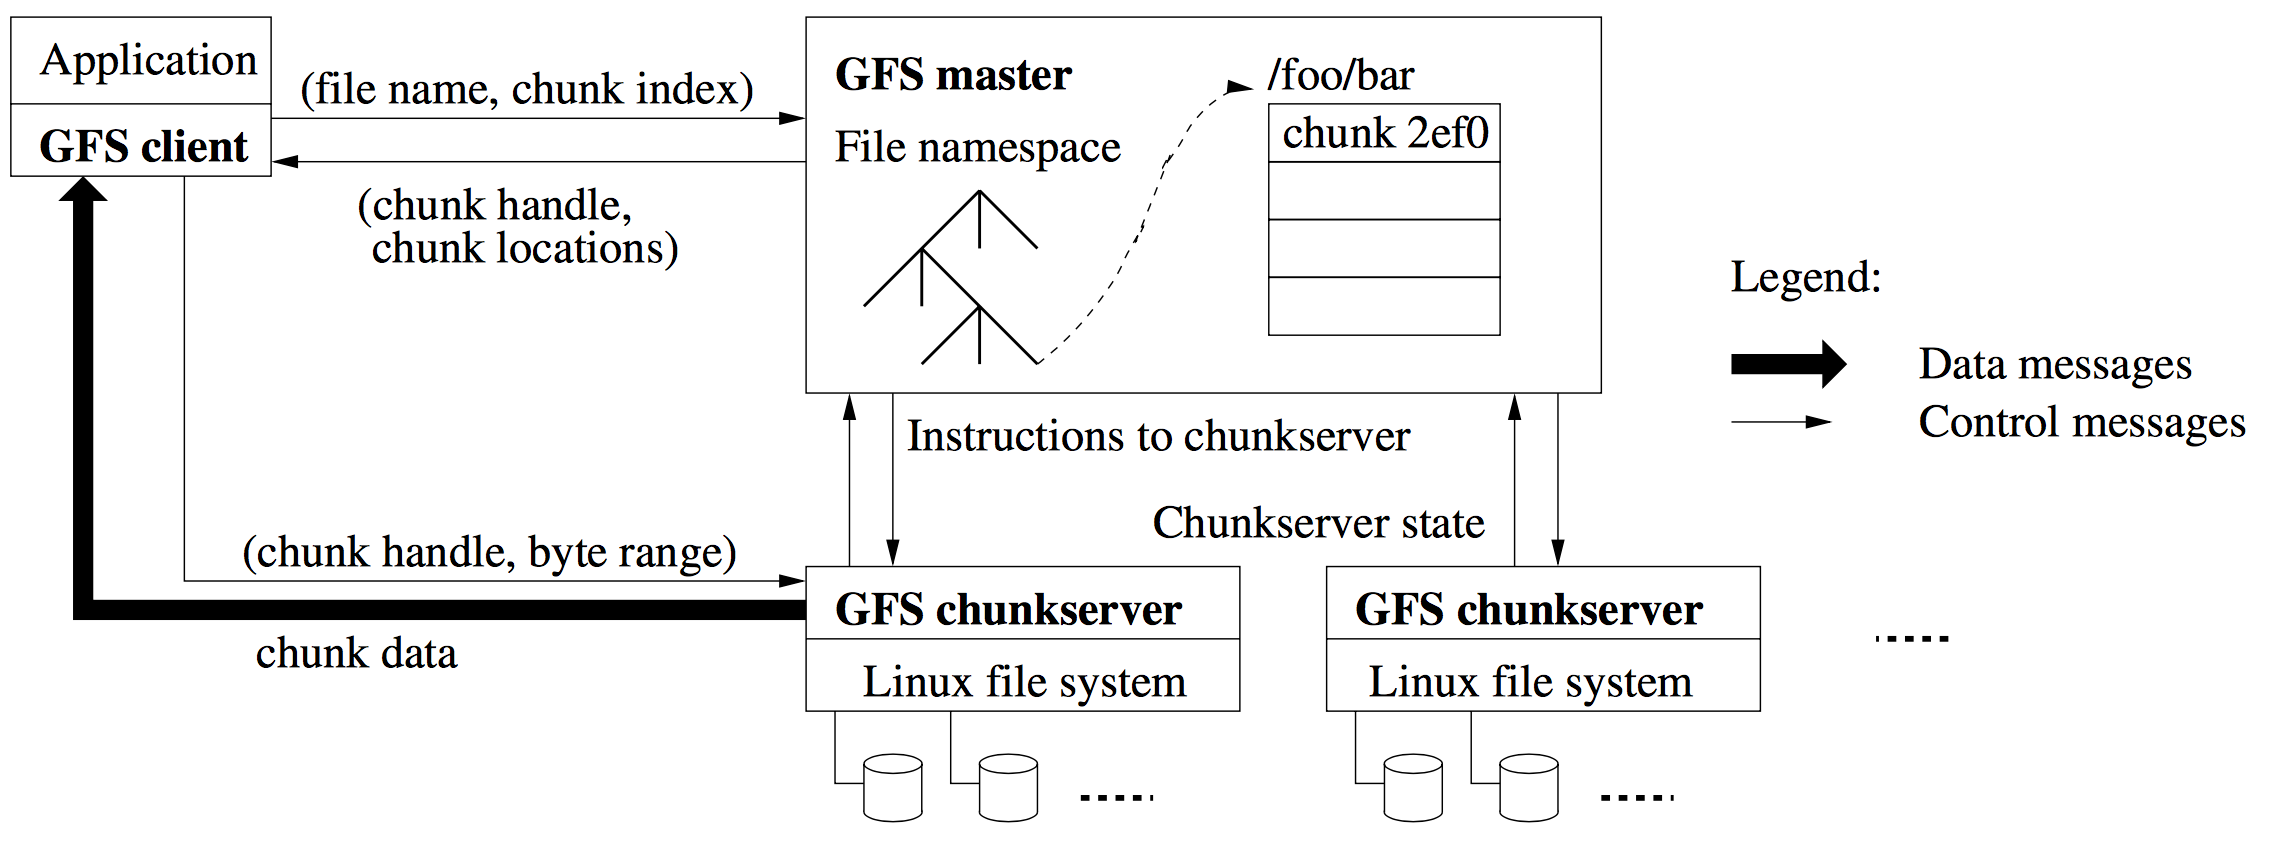
\includegraphics[width=\linewidth]{GFS.png}
\end{figure}

%--------------
\subsubsection{MapReduce: A Framework for Parallel Programming}
\begin{itemize}
\item Minimize effort of programmer for simple parallel processing tasks
\begin{itemize}
\item Features
\item Hide many low-level details (network, storage) 
\item Built-in fault tolerance
\item Automatic load balancing
\end{itemize}
\end{itemize}


%--------------
\subsubsection{MapReduce: Computation Pipeline}
\begin{figure}[H]
    \centering
    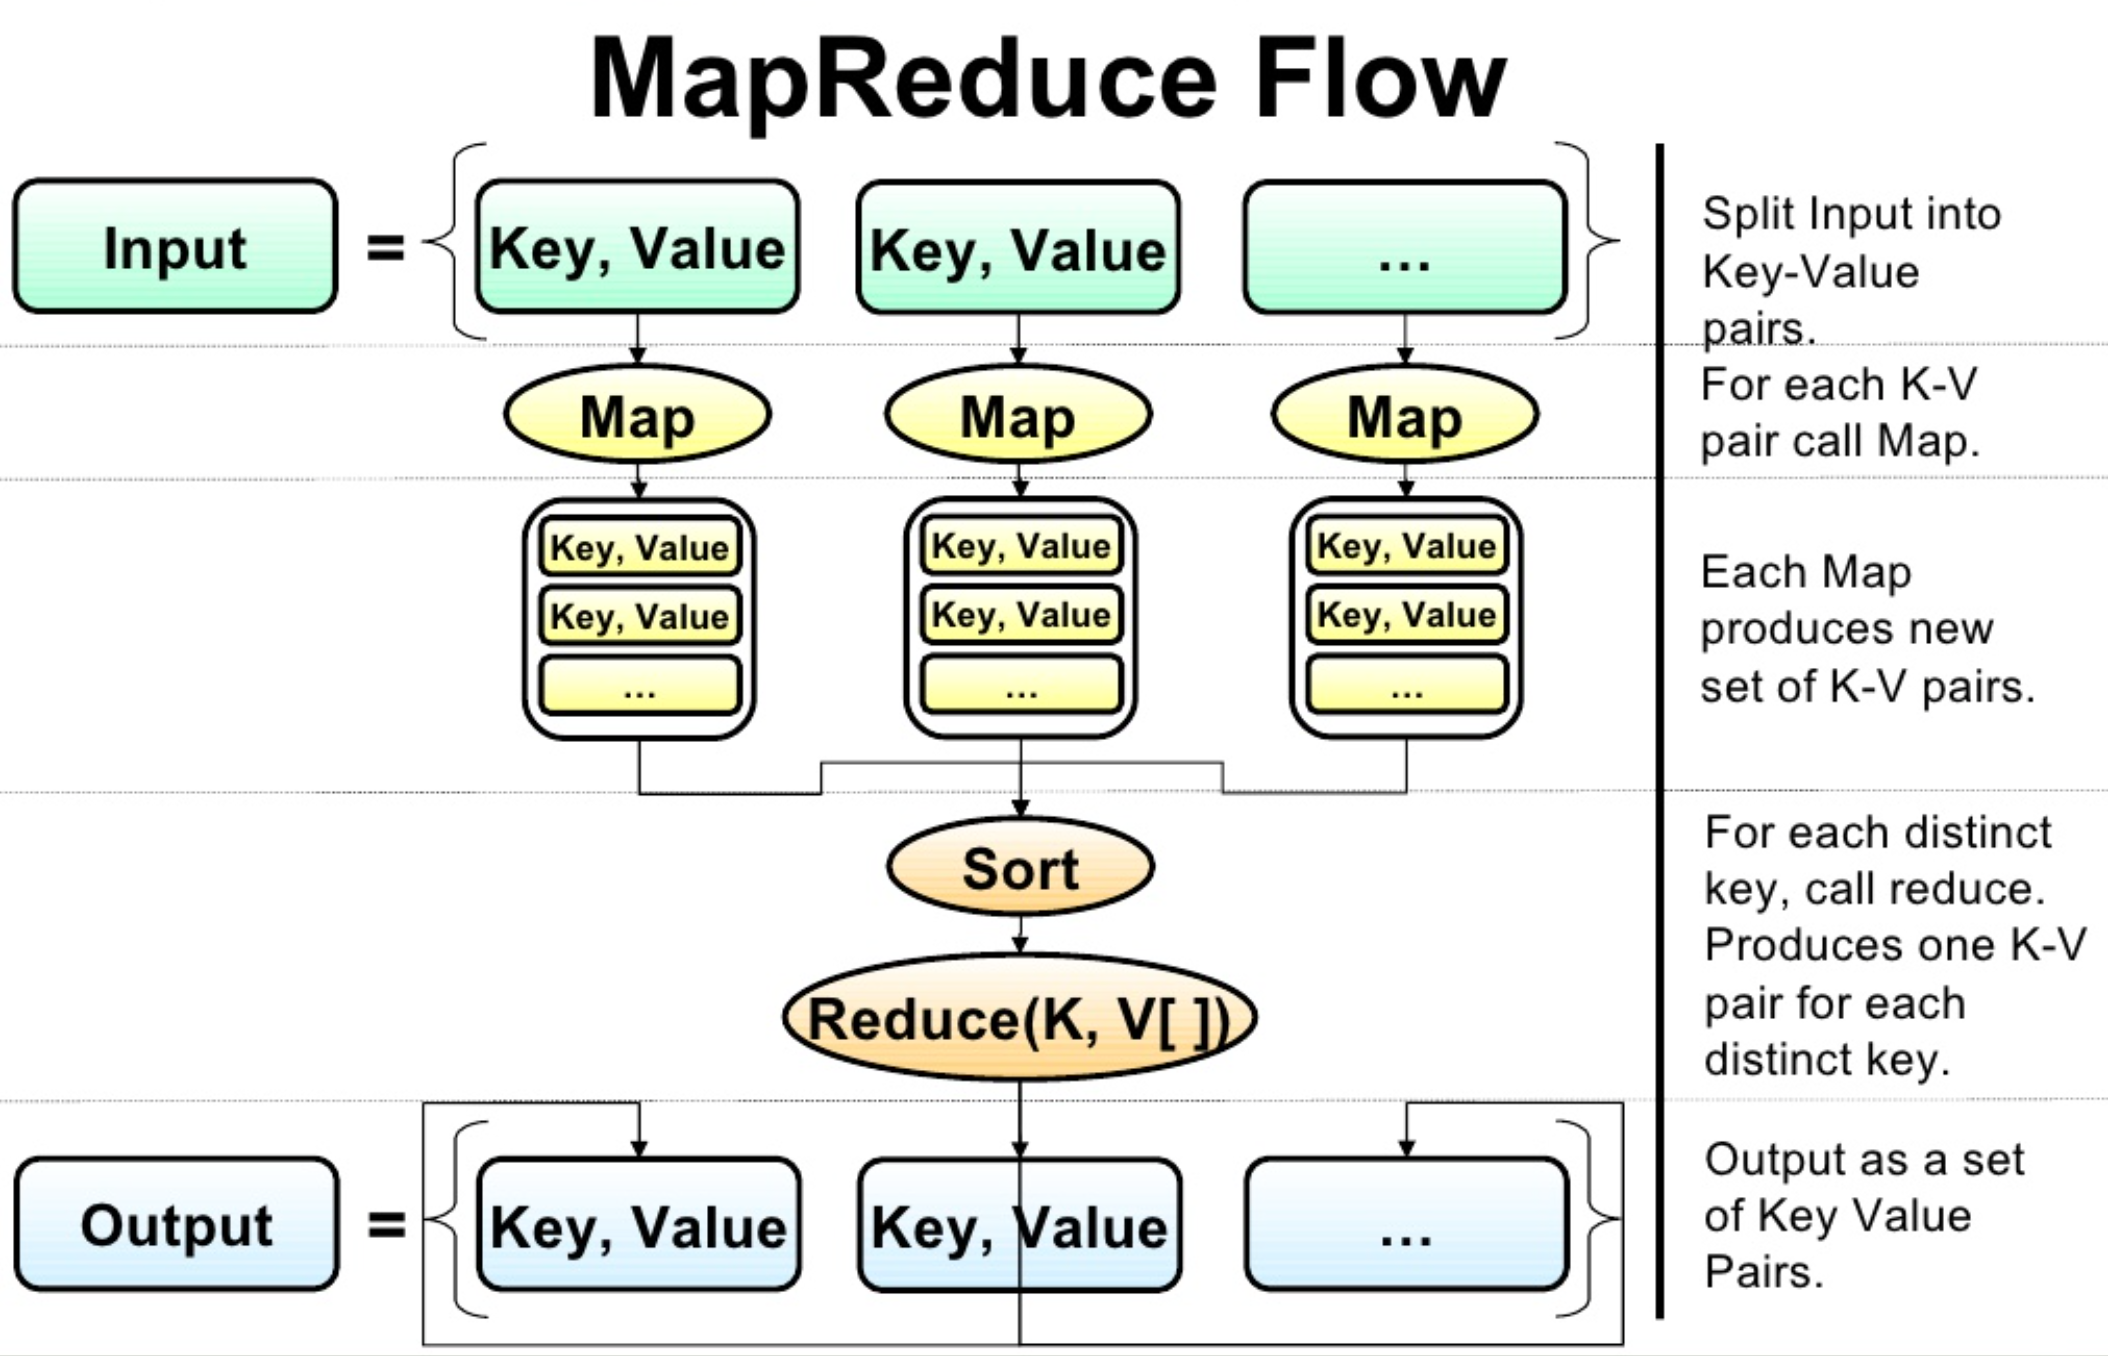
\includegraphics[width=\linewidth]{map_reduce.png}
\end{figure}


%--------------
\subsubsection{Inverted Indexing with MapReduce}

\begin{figure}[H]
    \centering
    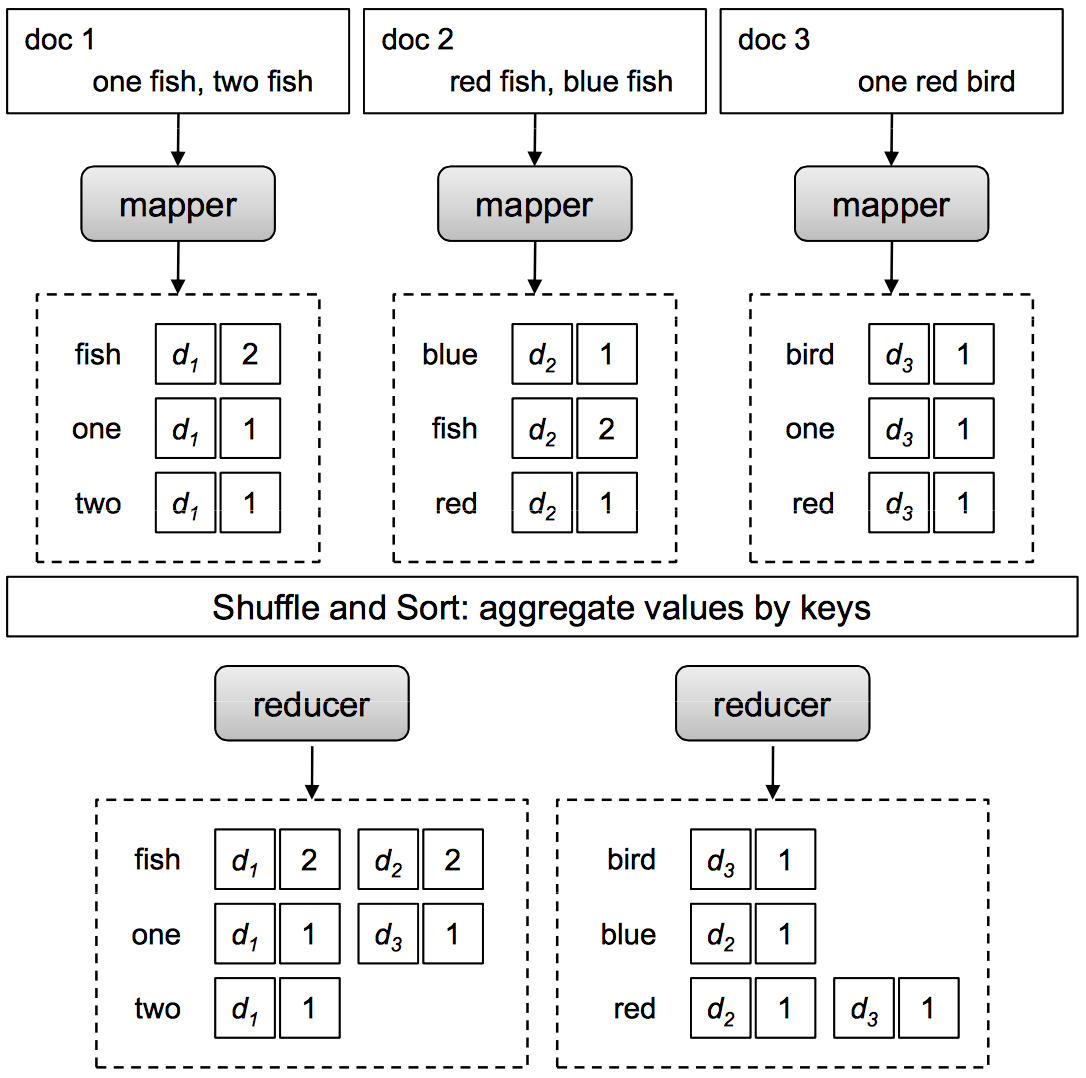
\includegraphics[width=0.8\linewidth]{mapreduce_inverted_index.png}
\end{figure}


\begin{algorithm}
\caption{Pseudo-code of the baseline inverted indexing algorithm in MapReduce}
\begin{algorithmic}
\State \textbf{class} Mapper
    \Procedure {Map}{docid $n$, doc $d$}
        \State $H \gets$ new AssociativeArray
        \ForAll {term $t \in$ doc $d$} 
            \State $H\{T\} \gets H\{T\}+1$
        \EndFor
        \ForAll {term $t \in H$}
            \State Emit(term $t$, posting $\langle n, H\{t\} \rangle$)
        \EndFor
    \EndProcedure  
    
    \State
\State \textbf{class} Reducer
    \Procedure{Reduce}{term $t$, postings $[\langle n_1, f_1 \rangle, \langle n_2, f_2 \rangle \dots]$}
        \State $P \gets$ new List
        \ForAll {posting $\langle a,f \rangle \in$ postings $[\langle n_1, f_1 \rangle, \langle n_2, f_2 \rangle \dots]$}
            \State Append($P$, $\langle a,f \rangle$) 
        \EndFor
        \State Sort($P$)
        \State Emit(term $t$, postings $P$)         
    \EndProcedure           
\end{algorithmic}
\end{algorithm}



%---------------------------------------------
\subsection{Link Analysis}

\subsubsection{Ranking Algorithms for Web Search}
\begin{itemize}
\item Standard IR models apply but aren’t sufficient 
\begin{itemize}
\item Different information needs (search for a particular web page instead of text information)
\item Documents have additional information (links, layout)
\item Information quality varies a lot
\end{itemize}

\item Major extensions
\begin{itemize}
\item Exploiting links to improve scoring
\item Exploiting clickthroughs for massive implicit feedback
\item In general, rely on machine learning to combine all kinds of features
\end{itemize}
\end{itemize}


%--------------
\subsubsection{Exploiting Inter-Document Links}

Description of a link (\textbf{<<anchor text>>}) is a summary and a query example for a target document.\\

An \textbf{authority} is a web page containing valuable information with respect to a specific subject. A \textbf{hub} is a web page not actually authoritative in the information it holds, but contains useful links toward an authoritative page – basically, advertising the authoritative web page.

\begin{figure}[H]
    \centering
    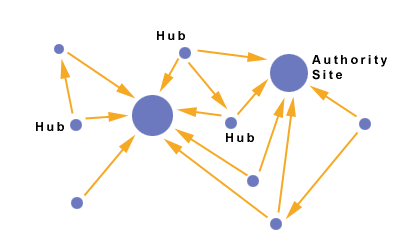
\includegraphics[width=0.8\linewidth]{hubs_and_authorities.png}
\end{figure}


%--------------
\subsubsection{PageRank: Capturing Page <<Popularity>>}
\begin{itemize}
\item Intuitions
\begin{itemize}
\item Links are like citations in literature
\item A page that is cited often can be expected to be more useful in general
\end{itemize}

\item PageRank is essentially <<citation counting>>, but improves over simple counting
\begin{itemize}
\item Consider <<indirect citations>> (being cited by a highly cited paper counts a lot...)
\item Smoothing of citations (every page is assumed to have a non-zero pseudo citation count)
\end{itemize}

\item PageRank can also be interpreted as random surfing (thus capturing popularity)
\end{itemize}


%--------------
\subsubsection{The PageRank Algorithm}

\begin{multicols}{2}
\begin{figure}[H]
    \centering
    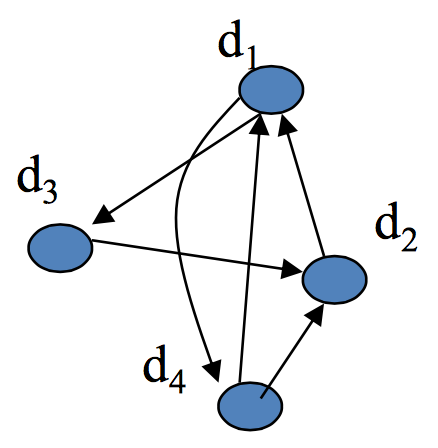
\includegraphics[width=0.7\linewidth]{page_rank_example.png}
\end{figure}


Transition matrix:
\begin{equation*}
M = 
\begin{pmatrix}
 0  &  0  & 1/2 & 1/2 \\
 1  &  0  &  0  &  0 \\
 0  &  1  &  0  &  0 \\
1/2 & 1/2 &  0  &  0 
\end{pmatrix}
\end{equation*}

$M_{ij}$ - probability of going from $d_i$ to $d_j$:

\begin{equation*}
\forall i: \sum_{j=1}^{N} M_{ij} = 1
\end{equation*}
\end{multicols}

\vspace{5mm}
<<Equilibrium Equation>>:
\begin{equation*}
p_{t+1}(d_j) = (1-\alpha) \sum_{i=1}^{N}M_{ij}\:p_t(d_i) + \alpha \sum_{i=1}^{N}\frac{1}{N}\:p_t(d_i),
\end{equation*}
where 
\begin{itemize}
\item $N$ - number of pages
\item $p_t(d_i)$ - probability of visiting page $d_i$ at time $t$
\item $\alpha$ - probability of jumping to a random page
\end{itemize}

\vspace{5mm}
For a converged\footnote{Converge - сходиться} state we can drop the time index:
\begin{equation*}
p(d_j) = \sum_{i=1}^{N} \left[ \frac{1}{N} \: \alpha + (1-\alpha) M_{ij} \right ] p(d_i) 
\end{equation*}
and come to this equation:
\begin{equation*}
\vec{p} = \Big(\alpha I + (1-\alpha) M \Big)^T \; \vec{p}, \text{ where } I_{ij} = \frac{1}{N},
\end{equation*}
which can be solved with an iterative algorithm starting with initial value $p(d)=1/N$.  

%--------------
\subsubsection{PageRank in Practice}
\begin{itemize}
\item Computation can be quite efficient since M is usually sparse
\item Normalization doesn’t affect ranking, leading to some variants of the formula

\item The zero-outlink problem: $p(d_i)$’s don’t sum to 1
\begin{itemize}
\item One possible solution = page-specific damping factor\footnote{Damping factor - коэффициент затухания}
($\alpha=1.0$ for a page with no outlink)
\end{itemize}
\item Many extensions (e.g., topic-specific PageRank)
\item Many other applications (e.g., social network analysis)
\end{itemize}


%--------------
\subsubsection{HITS: Capturing Authorities \& Hubs}
\begin{itemize}
\item Intuitions
\begin{itemize}
\item Pages that are widely cited are good authorities 
\item Pages that cite many other pages are good hubs
\end{itemize}

\item The key idea of HITS (Hypertext-Induced Topic Search) 
\begin{itemize}
\item Good authorities are cited by good hubs
\item Good hubs point to good authorities
\item Iterative reinforcement...
\end{itemize}

\item Many applications in graph/network analysis
\end{itemize}


%--------------
\subsubsection{The HITS Algorithm}

\begin{multicols}{2}
\begin{figure}[H]
    \centering
    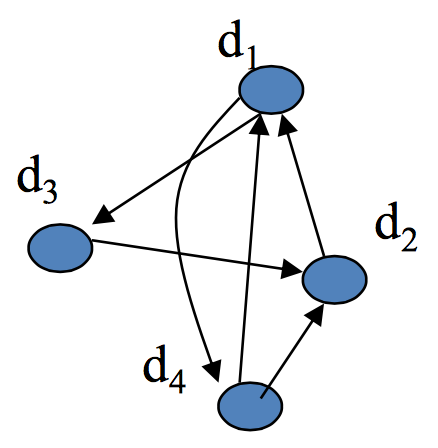
\includegraphics[width=0.7\linewidth]{page_rank_example.png}
\end{figure}


<<Adjacency matrix>>\footnote{<<Adjacency matrix>> $\approx$ матрица связей (<<соседства>>)}:
\begin{equation*}
A = 
\begin{pmatrix}
 0  &  0  &  1  &  1 \\
 1  &  0  &  0  &  0 \\
 0  &  1  &  0  &  0 \\
 1  &  1  &  0  &  0 
\end{pmatrix}
\end{equation*}


Algorithm:
\begin{itemize}
\item Initial values: $a(d_i)=h(d_i)=1$
\item Iteration:
\begin{equation*}
\begin{cases}
h(d_i) = \sum_{d_j \in OUT(d_i)} a(d_j) \\
a(d_i) = \sum_{d_j \in IN(d_i)} h(d_j)
\end{cases}
\end{equation*}
\item Iteration in matrix form:
\begin{equation*}
\begin{cases}
\vec{h} = A\,\vec{a} = AA^T\,\vec{h} \\
\vec{a} = A^T\,\vec{h} = A^TA\,\vec{a}
\end{cases}
\end{equation*}
\item Normalize: $\sum_i a(d_i)^2 = \sum_i h(d_i)^2 = 1$
\end{itemize}

\end{multicols}


%---------------------------------------------
\subsection{Learning to Rank}
%--------------
\subsubsection{How Can We Combine Many Features?}
\begin{itemize}
\item Given a query-doc pair $(Q,D)$, define various kinds of features
$X_i(Q ,D)$
\item Examples of feature:
\begin{itemize}
\item the number of overlapping terms, 
\item BM25 score of $Q$ and $D$, 
\item $p(Q \,\big|\, D)$, 
\item PageRank of $D$, 
\item $p(Q \,\big|\, D_i)$, where $D_i$ may be anchor text or big font text, 
\item <<does the URL contain ‘~’?>> 
\item etc.
\end{itemize}
\item Hypothesize $p(R=1 \,\big|\, Q, D) = s\big( X_1(Q,D), \dots ,X_n(Q,D), \lambda \big)$, where $\lambda$ is a set of parameters
\item Learn $\lambda$ by fitting function s with training data, i.e., 3-tuples like $(D, Q, 1)$ ($D$ is relevant to $Q$) or $(D,Q,0)$ ($D$ is non-relevant to $Q$)
\end{itemize}

%--------------
\subsubsection{Regression-Based Approaches}

Logistic Regression: 
\begin{itemize}
\item $X_i(Q,D)$ is feature
\item $\beta$’s are parameters
\end{itemize}

\begin{eqnarray*}
\log\frac{p(R=1 \,\big|\, Q, D)}{1-p(R=1 \,\big|\, Q, D)}=\beta_0 + \sum_{i=1}^{N} \beta_i X_i \\
p(R=1 \,\big|\, Q, D) = \frac{1}{1+\exp(-\beta_0 - \sum_{i=1}^{N} \beta_i X_i)}
\end{eqnarray*}

Estimate $\beta$’s by maximizing the likelihood of training data:
\begin{equation}
\vec{\beta}^* = \argmax_{\vec{\beta}} \, p \Big( \big\{ (Q_1, D_{11}, R_{11}), (Q_1, D_{12}, R_{12}), \dots , (Q_n, D_{n1}, R_{n1}), \dots \big\} \Big)
\end{equation}


%--------------
\subsubsection{More Advanced Learning Algorithms}
\begin{itemize}
\item Attempt to directly optimize a retrieval measure (e.g. MAP, nDCG)
\begin{itemize}
\item More difficult as an optimization problem 
\item Many solutions were proposed [Liu 09]
\end{itemize}

\item Can be applied to many other ranking problems beyond search
\begin{itemize}
\item Recommender systems
\item Computational advertising 
\item Summarization
\end{itemize}
\end{itemize}


%----------------------------------------
\subsubsection{Recommended reading}
\begin{itemize}
\item Tie-Yan Liu. <<Learning to Rank for Information Retrieval>>. Foundations and Trends in Information Retrieval 3, 3 (2009): 225-331.
\item Hang Li. <<A Short Introduction to Learning to Rank>>, IEICE Trans. Inf. \& Syst. E94-D, 10 (Oct. 2011): n.p.
\end{itemize}


%---------------------------------------------
\subsection{Future of Web Search}

\subsubsection{Next Generation Search Engines}
\begin{itemize}
\item More specialized/customized (vertical search engines):
\begin{itemize}
\item Special group of users (community engines, e.g., Citeseer) 
\item Personalized (better understanding of users)
\item Special genre/domain (better understanding of documents)
\end{itemize}

\item Learning over time (evolving)
\item Integration of search, navigation, and recommendation/filtering
(full-fledged information management)
\item Beyond search to support tasks (e.g., shopping)
\item Many opportunities for innovations!
\end{itemize}


\subsubsection{Future Intelligent Information Systems}
\begin{itemize}
\item Search $\Rightarrow$ Access $\Rightarrow$ Mining $\Rightarrow$ Task support
\item Keyword queries $\Rightarrow$ Search history $\Rightarrow$ Complete user model
\item Bag of words $\Rightarrow$ Entities-Relations $\Rightarrow$ Knowledge presentation
\end{itemize}












